\chapter{Definição do Modelo FEC} %Metodologia
\label{cap:abordagem}

    O projeto de sistemas de Inteligência Ambiental complexos (sistemas \acrshort{ami}), compostos por outros sistemas menores, é uma tarefa complexa que exige um alto grau de planejamento. A falha do desenvolvedor em enxergar, de forma correta, o resultado das interações entre os diversos componentes projetados para o sistema pode causar perdas na qualidade do serviço a ser ofertado e, ainda, desperdício de tempo/dinheiro para corrigir erros na etapa de implementação. Essa tarefa fica ainda mais complexa à medida que o sistema cresce em número de componentes e, consequentemente, de interações entre eles, principalmente se a aplicação tiver um caráter inovador e original.

    A engenharia de sistemas define uma série de métodos, ilustrados no diagrama V na Figura \ref{fig:systems-vee}, que podem auxiliar no projeto e no teste dos sistemas \acrshort{ami}. A parte da descida do modelo V, que diz respeito às etapas aconselhadas para o projeto, compreende a definição dos conceitos da aplicação, sendo elas: análise de requisitos, análise funcional e a síntese do projeto. Em seguida, durante a etapa de implementação, a parte da subida do modelo V orienta a definição e execução de diversos tipos de testes, verificação e validação do sistema projetado. 

    A abordagem proposta neste capítulo consiste em uma contribuição à etapa de análise funcional do sistema. Permitindo o estudo de \textit{feedbacks} para refinar as etapas de análise de requisitos e de síntese do projeto. Mais especificamente, a abordagem permitirá ao projetista realizar estudos experimentais, visando verificar/encontrar decomposições funcionais alternativas de subsistemas componentes capazes de atender aos requisitos funcionais e de desempenho do sistema \acrshort{ami}. 
    
    Como resultados, tais estudos poderão indicar ao projetista a necessidade de se revisar a etapa de análise de requisitos para resolver problemas funcionais. Isso pode levar a mudanças na etapa de síntese de projeto e, consequentemente, na busca de uma arquitetura física adequada, em termos de componentes de \textit{hardware} e de \textit{software} componentes do sistema. 
    
    A ideia principal da abordagem está em representar, formalmente, determinadas decomposições funcionais do sistema \acrshort{ami} através de organizações de programas de agentes artificiais. Em seguida, utilizar uma plataforma de simulação multiagente adequada ao formalismo proposto, que permita ao projetista entender melhor o comportamento do sistema \acrshort{ami} em projeto, analisando seu desempenho em diferentes cenários do ambiente de tarefas, prevenindo erros e auxiliando a construção de projetos mais eficientes. A abordagem propõe um quadro formal para o projetista empregar na representação das organizações de programas em seus aspectos funcionais, estruturais e comportamentais.
    
    As duas próximas seções apresentam a abordagem proposta. A Seção \ref{sec:pontos-propostas} define como o projetista deve enxergar o sistema \acrshort{ami} para que ele possa ser representado por uma organização de programas de agentes racionais. A Seção \ref{subsec:desc-fec} descreve o quadro formal, denominado modelo \acrshort{fec}. Finalmente, o Capítulo \ref{cap:resultados} descreve como organizações, formalizadas por meio do modelo \acrshort{fec}, podem ser executadas em uma plataforma de simulação multiagente permitindo a observação do desempenho de um sistema \acrshort{ami} associado à medida que os programas interagem entre si e com um ambiente de tarefas simulado.
    
\section{Principais Pontos de Vista e Propostas na Abordagem}
\label{sec:pontos-propostas}

Esta seção descreve os principais pontos de vista e propostas na abordagem para ajudar no projeto de sistemas \acrshort{ami}. São elas: 

\begin{itemize}
    \item[\textbf{P1} -] Definição de sistema de Inteligência Ambiental (sistema \acrshort{ami}) como um conjunto formado por um sistema técnico que interage com um ambiente de tarefas contendo pessoas, visando realizar algum objetivo original.
    
    \item[\textbf{P2} -] Definição de sistema técnico como um composto de \textit{hardware} e \textit{software}, onde cada um de seus elementos pode ser representado por um agente artificial. Composto de uma arquitetura e um programa de agente.
    
    \item[\textbf{P3} -] Descrição informal de um sistema \acrshort{ami} por meio de uma organização de programas de agentes racionais, para representar tanto o \textit{software} quanto o \textit{hardware} e as pessoas usuárias do sistema técnico. 
    
    \item[\textbf{P4} -] Descrição informal de uma organização com muitos programas de agentes interagindo em pelo menos dois níveis diferentes de aprofundamento/especificação.
    
    \item[\textbf{P5} -] Descrição formal da organização de programas de agentes, representando o sistema \acrshort{ami} em seus aspectos funcionais (modelo $F$), estruturais (modelo $E$) e comportamentais (modelo $C$) – modelo $FEC$ da organização.
    
    \item[\textbf{P6} -] Utilização de estratégias de simulação baseada em agentes e a noção de objetos emergentes, que são medidas (distribuições) associadas ao desempenho do sistema técnico e de cada um de seus subsistemas componentes, previamente formalizados em um modelo \acrshort{fec} de uma organização de programas de agentes, como meio de avaliar o desempenho de um sistema em projeto em um ambiente de tarefas virtual.
    
    \item[\textbf{P7} -] Execução de simulações que permitam ao projetista entender como os efeitos da aleatoriedade das ações (falhas), de alguns componentes do sistema interferem na forma e nas propriedades macro de uma distribuição.
    
    \item[\textbf{P8} -] Simulação das condições de atuação do sistema técnico e das pessoas no ambiente real do sistema \acrshort{ami}. Simulação do comportamento dessas pessoas em programas de agentes na organização representando pessoas.
    
    \item[\textbf{P9} -] Definição da noção de caso de teste para avaliar o desempenho de um sistema \acrshort{ami} em projeto, como sendo qualquer configuração particular do ambiente de tarefas simulado. Ainda, um conjunto de casos de teste descreve diferentes configurações ambientais, isto é, problemas de diferentes níveis de dificuldade para o sistema, que permitem ao projetista entender e dominar os mecanismos que causam a emergência de diversas distribuições associadas aos componentes do sistema técnico.
    
\end{itemize}

    Mais explicitamente, a proposta \textbf{P1} considera que um sistema de Inteligência Ambiental (sistema \acrshort{ami}) é composto por um sistema técnico e pelo sistema ambiental. O sistema técnico trata de todo o conjunto \textit{hardware}/\textit{software}, tais como: sensores, atuadores, artefatos computacionais, serviços e aplicações de software. Em aplicações \acrshort{ami}, o sistema técnico deve, de maneira não intrusiva, perceber informações de seu ambiente de tarefa, e, a partir delas, selecionar ações a serem executadas.    
    
    O sistema ambiental é composto por tudo que foge do controle do projetista na aplicação, ou seja, as pessoas e o próprio ambiente. Dessa forma, o sistema técnico interage com o ambiente e com as pessoas que circulam por ele, buscando realizar algum objetivo original (função global do sistema). A Figura \ref{fig:sistema-tec-p1} ilustra a ideia de um sistema \acrshort{ami} visto como um composto integrado de pessoas e um sistema técnico composto por duas partes principais. 

   
    \begin{figure}[h!]
        \centering
        \Caption{\label{fig:sistema-tec-p1} Separação do sistema \acrshort{ami} em sistema técnico e ambiental.} 
        \UECEfig{}{
            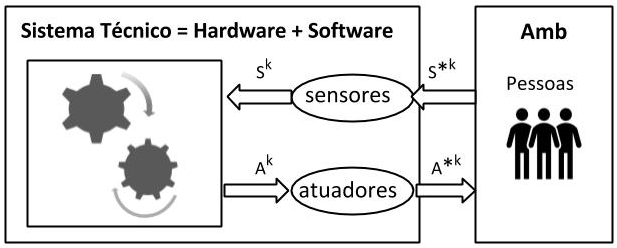
\includegraphics[width=8cm]{figuras/sistema-tec-p1}
        }{
            \Fonte{Elaborada pelo autor.}
        }   
    \end{figure}
    
    Muitos sistemas técnicos atuais são distribuídos e envolvem uma interação complexa entre pessoas e máquinas. Por exemplo, pode-se imaginar o \textit{hardware} em um ambiente semelhante a um prédio, incluindo os sensores e atuadores, e o \textit{software} para monitorar e controlar o \textit{hardware} no prédio, visando satisfazer as pessoas, por exemplo, adaptando a temperatura e a intensidade da luz de acordo com as preferências destas pessoas, e gastando o mínimo de energia possível, por exemplo, desligando automaticamente as lâmpadas e o ar-condicionado de salas vazias.
    
    A proposta \textbf{P2}, em resumo, considera que o sistema técnico da aplicação \acrshort{ami} pode ser representado por um ou mais agentes artificiais. Isto é, um sistema formado por uma arquitetura, ou seja, algum tipo de dispositivo computacional com sensores e atuadores físicos, e por um programa de agente que implementa a função do agente, e mapeia percepções em ações. A arquitetura disponibiliza ao programa as percepções de seus sensores. O programa é executado para selecionar as ações de acordo com as informações recebidas. E, por fim, as ações são executadas pelos atuadores definidos na arquitetura. Cada programa de agente pode incorporar uma série de componentes funcionais associados à (\emph{subsistemas}) percepção (\emph{ver}), atualização de estado interno (\emph{próximo}) e tomada de decisão (\emph{ação}).
    
    Assim, de acordo com a abordagem, qualquer sistema técnico poderá ser abstraído pela noção de agente artificial. Podem ser sistemas simples, como um ar-condicionado com controle inteligente, um robô mais sofisticado para prestar serviços de interesse das pessoas, ou mesmo um sistema técnico complexo, composto de vários subsistemas (agentes artificiais) conectados por um modelo de cooperação/competição, onde cada subsistema pode usar funcionalidades de outros para compensar ou complementar a sua própria funcionalidade, visando realizar o objetivo original do sistema \acrshort{ami}.
    
    Com relação às duas primeiras propostas: a proposta \textbf{P3} considera que o sistema \acrshort{ami} pode ser descrito informalmente como uma organização de programas de agentes capazes de representar tanto o \textit{software} ($AgSoftware$) quanto o comportamento de grande parte do \textit{hardware} ($AgHardware$) que compõe a arquitetura do sistema técnico, e, ainda, das pessoas usuárias ($AgPessoas$) deste sistema. A Figura \ref{fig:org-agentes-p3} ilustra tal ideia, considerando a ideia de sistema \acrshort{ami} na Figura \ref{fig:sistema-tec-p1}.
    
    \clearpage
    \begin{figure}[h!]
        \centering
        \Caption{\label{fig:org-agentes-p3} Representação dos componentes de um sistema \acrshort{ami} como agentes inteligentes.} 
        \UECEfig{}{
            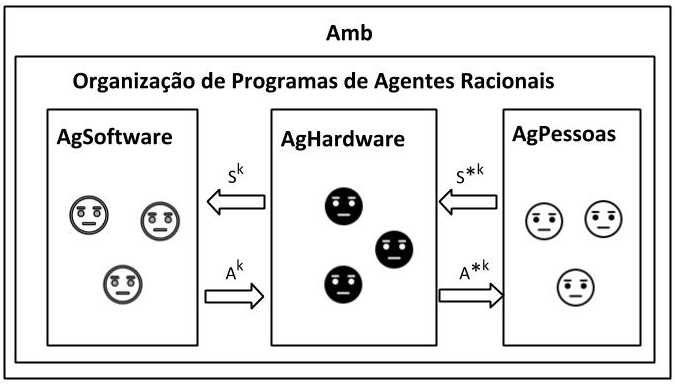
\includegraphics[width=8cm]{figuras/org-agentes-p3.png}
        }{
            \Fonte{Elaborado pelo autor.}
        }   
    \end{figure}
    
    Ou seja, além de definir o \textit{software} do sistema ($AgSoftware$) como programas de agentes, que seriam responsáveis por monitorar e controlar o \textit{hardware} do sistema, a abordagem propõe modelar tanto o comportamento dos usuários, quanto o desempenho dos sensores e atuadores definidos na arquitetura do sistema, utilizando programas de agentes racionais, respectivamente denominados $AgPessoas$ e $AgHardware$. À medida do possível, considerando essa generalização, a descrição informal deve indicar o esboço de uma estrutura e do comportamento desejado para o grupo de programas na organização. Eles devem ser adequados ao ambiente de tarefas e, consequentemente, ao alcance do objetivo original do sistema.
    
    Em \textbf{P4}, a proposta é que uma organização com muitos programas de agentes interagindo seja descrita informalmente em pelo menos dois níveis diferentes de aprofundamento/especificação. O objetivo é analisar e compreender melhor o sistema \acrshort{ami}, dessa forma: 
    
    \begin{itemize}
        
        \item Nível 1: a aplicação \acrshort{ami} abstraída é como uma única entidade formada por um sistema técnico (agente artificial), descrito por uma organização de programas de agentes composta por um único programa do tipo $AgSoftware$, que interage com pelo menos um programa de agente do tipo $AgHardware$ para representar sensores e atuadores capazes de interagir com um ambiente, que pode conter programas de agentes do tipo $AgPessoas$ (Figura \ref{fig:org-level-p4}a); 
        
        \item Nível 2:  a aplicação \acrshort{ami} é abstraída como uma entidade composta por vários sistemas técnicos (agentes artificiais) conectados. O sistema \acrshort{ami} é descrito por uma organização de organizações de programas de agentes, cada uma descrevendo um dos sistemas técnicos componentes (Figura \ref{fig:org-level-p4}b). 
    
    \clearpage
    \end{itemize}
    
    \begin{figure}[h!]
        \centering
        \Caption{\label{fig:org-level-p4} Diferentes níveis de abstração de um sistema \acrshort{ami}.} 
        \UECEfig{}{
            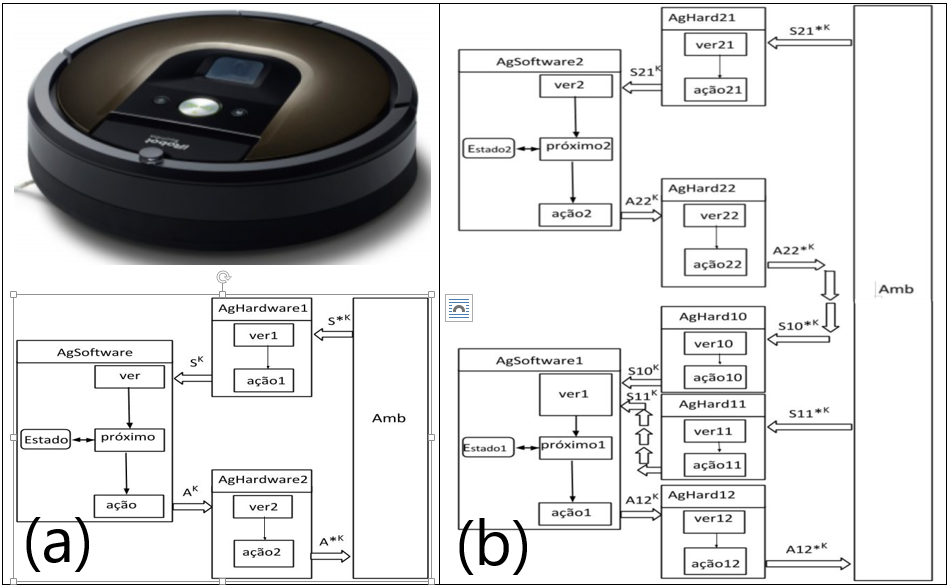
\includegraphics[width=10cm]{figuras/org-level-p4.png}
        }{
            \Fonte{Elaborado pelo autor.}
        }   
    \end{figure}
    
    Tomemos como exemplo uma aplicação de inteligência ambiental em que o sistema é responsável por manter o ambiente limpo enquanto pessoas transitam pelo ambiente. A Figura \ref{fig:org-level-p4}a ilustra a situação onde esse sistema \acrshort{ami} é modelado por um único sistema técnico, ou seja, um robô aspirador de pó. Descrito por uma organização composta por um programa de agente $AgSoftware$ capaz de controlar o aspirador de pó e dois programas de agente $AgHardware1$ e $AgHardware2$ para representar respectivamente um sensor e um atuador do sistema técnico no ambiente. No exemplo, enquanto o programa $AgSoftware$ é do tipo com estado interno, os programas $AgHardware1$ e $AgHardware2$ são do tipo reativo simples.
    
    Já a Figura \ref{fig:org-level-p4}b ilustra a situação desse mesmo sistema \acrshort{ami}, porém, modelado por dois sistemas técnicos. Agora, além do sistema técnico que representa os aspiradores de pó, temos um outro sistema para monitorar ambientes. Este utilizaria um conjunto de câmeras estáticas para reconstruir o estado do ambiente, incluindo a posição do robô aspirador de pó. O primeiro sistema técnico, o aspirador, descrito pela organização formada pelos programas $AgSoftware1$, $AgHard10$, $AgHard11$ e $AgHard12$, utiliza a funcionalidade de localização global gerada pelo segundo sistema técnico, o de monitoramento, descrito pela organização formada pelos programas $AgSoftware2$, $AgHard21$ e $AgHard22$, para selecionar uma estratégia mais inteligente de navegação e limpeza.
    
    A proposta em \textbf{P5} é que a organização de programas de agentes, representando o sistema \acrshort{ami}, seja especificada previamente em seus aspectos funcionais (modelo F), estruturais (modelo E) e comportamentais (modelo C), empregando um formalismo adequado. O modelo F proposto refere-se à descrição formal da função global (objetivo original) de uma parte da organização de programas representando o sistema técnico; o modelo E refere-se à descrição formal da estrutura visível da organização de programas representando o sistema \acrshort{ami}; e o modelo C refere-se à descrição formal dos processos que ocorrem dentro desta organização e, principalmente, como os programas de agentes representando o sistema técnico devem se comportar para alcançar os resultados desejados no ambiente de tarefas.
    
    Em seguida, a proposta \textbf{P6} recomenda utilizar simulação baseada em agentes e a noção de objetos emergentes como meio de avaliar o desempenho de um sistema em projeto, previamente formalizado em um modelo \acrshort{fec} de uma organização de programas de agentes. Mais especificamente, a abordagem propõe que as interações entre os programas na organização, e desta com o ambiente de tarefas, seja simulada durante um período de tempo. Assim, o desenvolvedor pode perceber se a estrutura, descrita no modelo $E$, e o comportamento integrado destas entidades, descrito no modelo $C$, funcionam de maneira a realizar o objetivo original do sistema, descrito no modelo $F$.
    
    Mais especificamente, a abordagem propõe a execução de simulações de modelos \acrshort{fec} em ambientes de tarefas virtuais, em diferentes configurações e devidamente programados em linguagem adequada. A partir das simulações são extraídos objetos emergentes que são medidas (distribuições) associadas ao desempenho do sistema técnico e de cada um de seus subsistemas componentes. Observando esses objetos emergentes, o desenvolvedor tem uma melhor noção da capacidade do sistema de cumprir seu objetivo original. A Figura \ref{fig:sim-emergente-p6} ilustra esta ideia.
        
    \begin{figure}[h!]
        \centering
        \Caption{\label{fig:sim-emergente-p6} Fluxo de extração dos objetos emergentes.} 
        \UECEfig{}{
            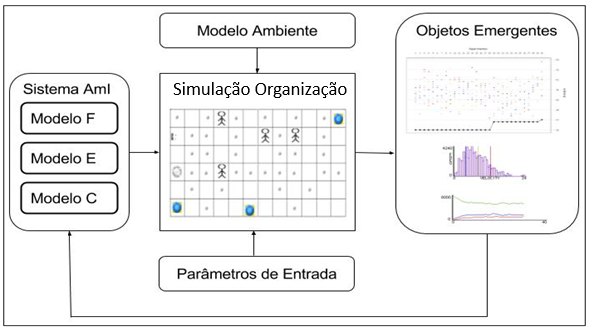
\includegraphics[width=10cm]{figuras/sim-emergente-p6.png}
        }{
            \Fonte{Elaborado pelo autor.}
        }   
    \end{figure}
    
    Assim, uma distribuição associada a um parâmetro de algum dos programas de agentes, componentes do sistema técnico, pode ser vista como uma descrição do que emerge das interações do sistema com seu ambiente de tarefas. Isso permite ao projetista avaliar as propriedades macro das distribuições associadas ao programa de agente, como, por exemplo: média, variância e desvio padrão. Como consequência, o desenvolvedor poderá dominar os mecanismos que causam a emergência desses objetos e utilizar a seu favor na economia de esforço e tempo para o desenvolvimento de um sistema \acrshort{ami} racional. 
    
    Nesse contexto, a proposta \textbf{P7} coloca em destaque particular o caso de ambientes de tarefas não determinísticos. A abordagem considera que o projetista deve buscar entender como os efeitos da aleatoriedade das ações de alguns componentes do sistema técnico interferem na forma e nas propriedades macro de uma distribuição. Este entendimento deve servir para garantir que os componentes de confiabilidade baixa, integrados e implementados em um sistema \acrshort{ami} realizarão o objetivo desejado em seu ambiente de tarefas.
    
    A proposta \textbf{P8} pode ser dividida em duas. Primeiro, a abordagem propõe que os programas de agentes $AgPessoas$ devem simular o comportamento dos usuários do sistema. Essa imitação deve ser suficiente para que o efeito de suas ações no ambiente simulado gere como resposta um comportamento correspondente adequado dos programas de agentes dos tipos $AgHardware$ e $AgSoftware$, representando o sistema técnico. Segundo, propõe também que o ambiente de tarefas virtual deve simular adequadamente as condições de atuação do sistema técnico e das pessoas no ambiente real. 
    
    Sabe-se que a natureza de qualquer ambiente de tarefa pode ser classificada de acordo com sete dimensões (propriedades), sendo elas: observável-parcialmente observável, determinístico-estocástico, episódico-sequencial, estático-dinâmico, discreto-contínuo, agente único-multiagente, e conhecido-desconhecido. Assim, a abordagem considera que, em conjunto com outros objetos presentes em um ambiente real, essas propriedades devem ser também adequadamente simuladas. 
    
    Finalmente, a proposta \textbf{P9}, considera que uma configuração particular do ambiente simulado define um caso de teste para o sistema \acrshort{ami} em projeto, e que diferentes configurações compreendem diferentes casos de testes, definindo problemas de diferentes níveis de dificuldade para o sistema. Por exemplo, considerando-se um sistema \acrshort{ami} composto por um sistema técnico formado por uma certa quantidade de robôs para atuar em um local semelhante a um aeroporto, uma configuração particular do ambiente deve definir o número de obstáculos, de lixo e de pessoas em locais específicos do aeroporto. Neste tipo de ambiente, algumas configurações podem exigir dos robôs maior consumo de energia, enquanto outras podem colocar lixo em locais de mais fácil acesso aos robôs.
    
\begin{section}{Modelo FEC de uma Organização de Programas}
\label{subsec:desc-fec}

    Conforme dito na introdução da seção anterior, para avaliar o alcance de um objetivo original por parte de um sistema \acrshort{ami} em projeto, o projetista deve considerar a relação existente entre três partes, sendo elas: (1) o objetivo original do sistema; (2) o seu ambiente interno, aqui representado por uma organização de programas de agentes; e (3) o ambiente de tarefas em que o sistema funciona. De acordo com a proposta, para concluir que o sistema \acrshort{ami} é adequado ao ambiente de tarefas, o projetista necessita comprovar primeiro que organização de programas alcança o objetivo original do sistema, então ele poderá concluir que o projeto do ambiente interno do sistema está caminhando na direção da adequação ao ambiente externo. 

    \citeonline{norvig2004inteligencia} enfatizam a importância de se especificar adequadamente a natureza dos ambientes de tarefas durante o projeto de sistemas compostos por agentes artificiais. Dependendo da natureza desses ambientes, o projetista pode entender a sua tarefa em diferentes graus de complexidade, variando desde problemas bem definidos, em ambientes de tarefas observáveis, determinísticos e estáticos, até problemas difíceis de exploração, em ambientes de tarefas parcialmente observáveis, não determinísticos, dinâmicos, desconhecidos e multiagentes competitivos. A literatura sobre o assunto disponibiliza diversas referências; elas apresentam diversos resultados de abordagens para sistemas de agentes artificiais em todos esses ambientes de tarefas.

    O modelo \acrshort{fec} aqui proposto visa permitir que o projetista formalize adequadamente o primeiro e segundo termos dessa relação, permitindo uma descrição matemática e computacional deles, dessa forma facilitando que as organizações de programas de agentes, associadas aos sistemas \acrshort{ami} em projeto, possam ser implementadas, simuladas e avaliadas quanto à realização do seu objetivo original. No que diz respeito à formalização da organização (2), o modelo \acrshort{fec} visa permitir que o projetista se concentre nas partes (estruturas) de uma organização, no entendimento de como estas partes funcionam (comportamentos) e o que fazem (funções). Nesse contexto, a simulação de um modelo \acrshort{fec} permitirá ao projetista perceber relações que podem não ser aparentes entre as estruturas possíveis. Os comportamentos e as funções de uma organização representando um sistema \acrshort{ami}.
    
    \subsection{Modelo de Função (F)}
    \label{modelo-fec-f}
    
    O modelo de Função ($F$) de uma organização refere-se à descrição formal da função global (objetivo original) do sistema \acrshort{ami} (ou de algum de seus subsistemas). Este modelo deve estar em sintonia com algumas das saídas da etapa de análise de requisitos, no processo de engenharia do sistema. Mais especificamente, o modelo $F$ permite que o projetista formalize os objetivos dos atores interessados e envolvidos com o processo, além de orientar o projetista com mais clareza na especificação do modelo estrutural (E) e do modelo comportamental ($C$) da organização de programas de agentes. Esta formalização permite que o projetista obtenha uma medida de satisfação do objetivo do sistema \acrshort{ami}, determinando o desempenho da organização interagindo com um ambiente de tarefas virtual. É a partir da especificação do modelo $F$ da organização que o projetista deve definir os objetos emergentes (medidas e distribuições) das simulações de interações da organização com o ambiente virtual, visando avaliar o desempenho dos componentes do sistema, especificados previamente na etapa de análise funcional.

    A proposta considera que alguns dos objetivos originais dos atores interessados no projeto, descrevem determinadas exigências em relação ao sistema \acrshort{ami} pretendido. Outros objetivos podem descrever funções relevantes do sistema, ou qualidades que o sistema pretendido deve alcançar ou fornecer. Voltando ao exemplo do aspirador de pó. Pode ser requisitado ao sistema que, além de manter um determinado local  (ambiente) limpo, ele deve também minimizar o uso dos recursos disponíveis utilizando, por exemplo, um \textit{software} de monitoramento e controle para otimizar a movimentação dos robôs.
    
    Os objetivos originais articulam as necessidades percebidas, desejos e requisitos a alcançar com as decisões relacionadas ao projeto do sistema \acrshort{ami}. Estes objetivos podem expressar generalidades (por exemplo: melhorar a qualidade dos serviços) e, frequentemente, não podem ser diretamente quantificados, necessitando maiores esclarecimentos em termos de objetivos próximos que sejam mensuráveis. Assim, o projetista deve definir formalmente tais objetivos próximos como substitutos do objetivo original, e seus valores de importância no contexto do objetivo original, indicando como os objetivos próximos contribuem com diferentes graus para a satisfação do objetivo original.
    
    Por exemplo, no caso do sistema \acrshort{ami} para limpeza de ambientes públicos mencionado, o projetista pode definir que o objetivo original ($O_0$) do sistema técnico consiste em prestar um serviço de alta qualidade, com um mínimo de despesas e o máximo de educação com as pessoas presentes no ambiente. Como consequência, de maneira a satisfazer o objetivo original do sistema, o projetista pode definir para os agentes aspiradores pelo menos quatro objetivos próximos possíveis de serem medidos, ou seja: manter o ambiente limpo ($O_1$), manter energia suficiente na bateria ($O_2$), trabalhar em equipe ($O_3$), e cumprimentar as pessoas ($O_4$).
    
    De acordo com o esquema de decomposição do objetivo original proposto, a ideia no modelo $F$ é de que o projetista deve definir, formalmente, o objetivo original do sistema \acrshort{ami} por meio de uma função de utilidade que considera: (1) um vetor de funções escalares associadas aos objetivos próximos; e (2) os valores de importância desses objetivos no contexto do objetivo original. Cada função escalar ($av_i$) no modelo $F$ associa valores no domínio dos números reais com um conjunto de episódios possíveis ($Ep$), descritos em termos de um conjunto de estados do ambiente (percepções $S$) e um conjunto de ações possíveis para o sistema ($A$).
    
    Por exemplo, a Tabela \ref{tab:asp-resultados} exemplifica alguns valores de satisfação/insatisfação nos objetivos próximos $O_1$ e $O_2$ (funções escalares $av_1$ e $av_2$), relacionados aos objetos emergentes de energia e limpeza, medidos em diversos episódios ($Ep_k$) na história das interações (k) mantidas por um programa de agente aspirador de pó em um ambiente de tarefas simulado. Os valores das funções indicam que cada agente artificial deve se movimentar e limpar um ambiente, maximizando os níveis de limpeza do ambiente e de energia em sua bateria ao final da tarefa.
    
    \begin{table}[h!]   
        \centering
        \Caption{\label{tab:asp-resultados} Histórico de ações do agente aspirador}
        \UECEtab{}{
            \begin{tabular}{ccclll}
                \toprule
                    $Ep^K $ & $S^K$ & $A^K$ & $av_1(Ep^K)$ & $av_2(Ep^K)$ \\
                \midrule \midrule
                  k  & \ldots L \ldots & asp & \phantom{-}0.0  & -1.0 \\
                  k+1  & \ldots L \ldots & les, oes, nor, sul  & \phantom{-}1.0  & -2.0 \\
                  k+2 & \ldots L \ldots & nop & \phantom{-}0.0  & \phantom{-}0.0 \\
                  k+3  & \ldots S \ldots & asp & \phantom{-}2.0  & \phantom{-}1.0 \\
                  k+4  & \ldots S \ldots & les, oes, nor, sul  & -1.0  & -2.0 \\
                  k+5  & \ldots S \ldots & nop & -1.0  & \phantom{-}0.0\\
                \bottomrule
            \end{tabular}
        }{
        \Fonte{Elaborado pelo autor}
    }
    \end{table}
        
    A segunda coluna ($S^k$) descreve uma parte das informações nas percepções do agente em cada episódio possível ($L$ = local limpo; $S$ = local sujo). A terceira coluna ($A_k$) descreve as ações possíveis para o agente nestes episódios ($asp$ = aspirar; $les$ = leste; $dir$ = direita; $oes$ = oeste; $nor$ = norte; $sul$ = sul; $nop$ = não operar). Na quarta e quinta colunas ($av_1$ e $av_2$), respectivamente associadas aos objetivos de limpeza ($O_1$) e de energia ($O_2$), estão as funções escalares para medir a satisfação dos objetivos pelo agente em cada episódio de sua história no ambiente de tarefas. 
    
    O restante desta seção formaliza as funções de avaliação e a função utilidade, componente principal do modelo F, que podem ser utilizadas para medir o desempenho de sistemas \acrshort{ami} do interesse do projetista. Ou seja, o modelo F permite que a performance de cada um dos agentes componentes do sistema e, mais especificamente, dos programas de agentes dos tipos $AgSoftware$ e $AgHardware$, componentes do sistema técnico, seja mensurada. Esses componentes podem ser identificados como $AgentAmI$ no quadro  formal abaixo. O quadro apresenta o esquema de representação e a definição correspondente dos principais termos envolvidos na definição da função utilidade:
    
    \begin{itemize}
        
        \item S = {$s_1$, $s_2$, \ldots} -- estados do ambiente do agente – em qualquer instante k o ambiente está em um dos estados do conjunto de estados do ambiente;
        
        \item A = {$a_1$, $a_2$, \ldots} -- capacidade efetuadora do agente – um conjunto de ações possíveis de serem executadas pelos atuadores do agente em qualquer instante k;
        
        \item ação : $S^*  \rightarrow A$ -- comportamento de um agente -- uma função que mapeia sequências de estados do ambiente $s \in S^*$ em ações $a \in A$, ou seja, intuitivamente, um agente decide que ação executar baseado em sua história, sua experiência até o momento da decisão;
        
        \item amb : $S\times A  \rightarrow S$ -- comportamento (determinístico) de um ambiente – uma função que mapeia o estado corrente do ambiente $s \in S$ e uma ação $a \in A$, em um estado $amb(s,a)$ resultantes da execução da ação $a$ no estado $s$;
        
        \item AgentAmI -- um programa de agente implementando concretamente a função ação de um dos agentes nos conjuntos de agentes $AgPessoas$, $AgHardware$ e $AgSoftware$;
        
        \item Amb -- um programa ambiente implementando a função amb, capaz de interagir com um programa AgentAmI por meio de algum protocolo de interação;
        
        \item $\Omega$ -- um conjunto de descrições de cenários de ambientes de tarefa factíveis de instanciar em Amb e avaliar AgentAmI;
        
        \item $Cenario_i \in \Omega$ -- uma descrição específica de cenário ambiental;
        
        \item $Cenarios \in P(\Omega$) -- um subconjunto de descrições de cenários ambientais (conjunto de casos de teste);
        
        \item $h(Cenario_i) \in (S\times A)N^{Int}$ -- história de comprimento $Nint$ de $AgentAmI$ em $Amb$ correspondente ao $Cenario_i \in \Omega$ – uma sequência $s_0 \xrightarrow{a_0} s_1 \xrightarrow{a_1} s_2 \xrightarrow{a_2} \ldots s_{Nint-1} \xrightarrow{a_{Nint-1}} s_(Nint)$, tal que $s_0$ é o estado inicial do ambiente, $a_{Nint-1}$ é a última ação que o agente escolheu para executar, e $s_{Nint}$ é o último estado do ambiente;
        
        \item $Ep^k(h(Cenario_i)) \in (S\times A)$ -- episódio na interação k, $k \leq Nint$, da história de $AgentAmI$ em $Amb$ correspondente ao caso $Cenario_i \in \Omega$;
    
        \item $H(Cenarios) \in P((S\times A)N^{Int})$ -- conjunto de histórias de comprimento $NInt$ de $AgentAmI$ em $Amb$ considerando $ProtocolInteracao$ e todos os cenários ambientais em $Cenarios \in P(\Omega)$;
    \end{itemize}
    
    Considerando o esquema de representação acima. O objetivo original a ser alcançado por um programa $AgentAmI$, em um ambiente de tarefas simulado por um programa $Amb$, pode ser formalizado por meio de um vetor de $M (M \geq 1)$ funções objetivo próximo (implícitas) do objetivo original estabelecido pelo projetista. Considerando um conjunto de cenários em H(Cenários), temos:

    \begin{equation}\label{eq:func-cen}
        f(H(Cenarios)) = f_1(H(Cenario), f_2(H(Cenario), \ldots, f_M(H(Cenario) \in R^M
    \end{equation}
        
    Supondo-se que o número de cenários no conjunto H(Cenários) seja $NCenarios$, a satisfação de um objetivo próximo $m (m = 1 \ldots M)$ alcançado por um $AgentAmI$ em $Amb$ pode ser formalizada:

    \begin{equation}\label{eq:func-cen-media}
        f_m(H(Cenarios)) = \frac{1}{NCenario} \sum_{i=1}^{NCenario} av_m(h(Cenario_i))
    \end{equation}

    Supondo-se que o comprimento de cada história do programa $AgentAmI$ em $Amb$ seja $NInt$, o valor medido de recompensa/penalização em um objetivo próximo m, alcançado pelo programa $AgentAmI$ em $Amb$ considerando o $Cenario_i \in \Omega$, pode ser formalizada: 
        
    \begin{equation}\label{eq:func-av}
        av_m(h(C_i)) = \sum_{k=1}^{Nint} av_m(Ep^k(h(Cenario_i)))
    \end{equation}
    
    tal que $av_m(Ep_k(h(Cenario_i)))$ é o valor medido de recompensa/penalização no objetivo próximo $m$ atribuído ao episódio $k$ da história associada ao $Cenario_i \in \Omega$. 
    
    Finalmente, a função Utilidade permitirá ao projetista obter medidas de desempenho de $AgentAmI$ em $Amb$ considerando um conjunto de cenários ambientais em $H(Cenarios)$. Supondo-se que o grau de utilidade de um objetivo próximo independe dos valores assumidos pelos demais (função é preferencialmente independente), este trabalho considera uma forma especial de função utilidade, ou seja, uma função aditiva no formato linear:
    
    \begin{equation}\label{eq:func-util}
        Utilidade(f(H(Cenarios))) = \sum_{m=1}^M w_m \cdot f_m(H(Cenario)))
    \end{equation}
    tal que $w_m \geq 0$, $m =1, \ldots, M$.
    
    Por exemplo, a Figura \ref{fig:func-objetivo-asp} ilustra os valores da função objetivo próximo de energia ($f_1$) e os valores de função utilidade, considerando também os valores de uma função objetivo próximo de limpeza ($f_2$), ao longo de cem, considerando dez cenários ambientais em cada um. 
    
    \begin{figure}[h!]
        \centering
        \Caption{\label{fig:func-objetivo-asp} Função objetivo em diversos cenários.} 
        \UECEfig{}{
            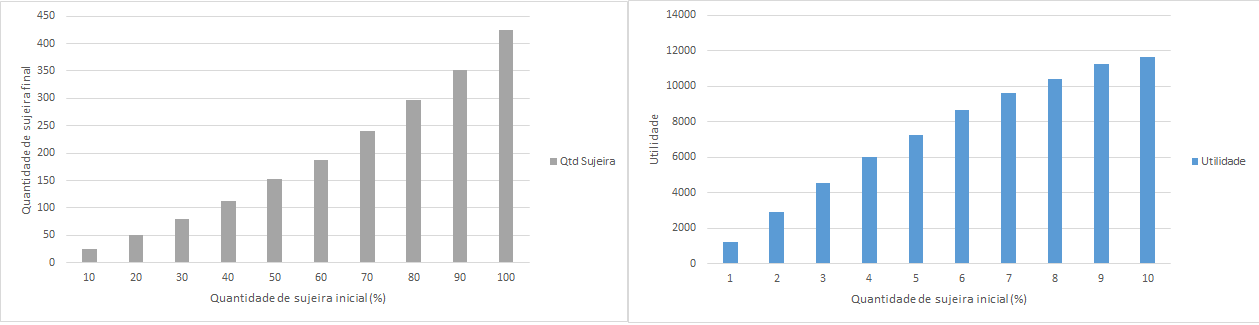
\includegraphics[width=14cm]{figuras/func-objetivo-asp-rob.png}
        }{
            \Fonte{Elaborado pelo autor.}
        }   
    \end{figure}

    Além de ajudar ao projetista a avaliar o desempenho de cada um dos programas de agentes artificiais em uma organização projetada, ou seja, dos subsistemas técnicos componentes do sistema técnico no sistema \acrshort{ami}, as medidas obtidas com estas funções de utilidade em simulações permitirão ao projetista realizar um julgamento a respeito do comportamento da organização de programas de agentes racionais em particular e, consequentemente, do próprio sistema \acrshort{ami} em projeto.
    
    \subsection{Modelo de Estrutura (E)}
    
    O projeto de uma estrutura organizacional de programas de agentes artificiais adequada a um ambiente de tarefas capaz de representar satisfatoriamente um sistema \acrshort{ami} em projeto é um problema combinatório complexo. Ainda mais considerando os muitos subsistemas técnicos, componentes e a quantidade de interações possíveis (conexões) entre eles. O projetista precisa montar e escolher uma estrutura adequada para o sistema, isto é, definir o número e os tipos de subsistemas, assim como quais subsistemas devem interagir entre si, de maneira que o comportamento resultante dessa integração seja adequado ao seu ambiente de tarefas, maximizando a função de utilidade que foi definida no modelo F da organização de programas de agentes representando o sistema. 
    
    Mais especificamente, o modelo E de uma organização de programas de agentes refere-se à descrição formal da sua estrutura. O modelo visa contribuir com a busca de soluções para o problema de projeto de estruturas organizacionais que possam ser facilmente testadas em simulações em computador. 
    
    O quadro formal que define o modelo E proposto pode ser dividido em duas partes. A primeira parte permite ao projetista definir o conjunto de programas de agentes, conjunto de papéis que esses programas podem assumir na organização e as relações entre esses papéis, além dos grupos de programas e a cardinalidade destes grupos. A segunda parte do modelo permite ao projetista definir o mapa das interações que ocorrem entre os programas de agentes em diferentes papéis dentro dos grupos que compõem a organização. O quadro abaixo apresenta o esquema de representação adotado e a definição correspondente dos principais termos componentes do modelo:
    
    \begin{itemize}
    
        \item Agents -- representa um conjunto de $N_A$ programas $AgentAmI$ na organização (lembrar que, no modelo $F$, $AgentAmI$ foi definido como um programa de agente implementando concretamente a função ação de um dos agentes nos conjuntos de agentes $AgPessoas$, $AgHardware$ e $AgSoftware$);
        
        \item Roles -- representa um conjunto de $N_R$ papéis que podem ser atribuídos aos programas de agentes $AgentAmI \in Agents$;
        
        \item AgentRoles -- uma família de $N_R$ conjuntos do tipo $AgentAmIR_j (j = 1 \ldots N_R)$, onde cada conjunto $AgentAmI_{Rj}$ é formado por $N_{Rj}$ programas $AgentAmI \in Agents$ desempenhando o papel $R_j \in Roles$;
        
        \item Groups -- uma família de NG conjuntos de programas de agentes, onde cada conjunto identifica um grupo de agentes exercendo seus papéis na organização;
        
        \item Bond -- uma família de relações do tipo $Bond_x(AgentAmI_{Ri}, AgentAmI_{Rj})$, onde cada relação $Bond_x(AgentAmI_{Ri}, AgentAmI_{Rj})$ representa uma relação binária de um tipo $x \in \{knowledge, control, coordination, authority\}$, existente entre os programas de agentes no conjunto $AgentAmIR_{i} \in AgentsRoles$ e os programas de agentes no conjunto $AgentAmIR_{j} \in AgentsRoles$, tal que para todo $Agent_1 \in AgentAmIR_{i}$ e todo $Agent_2 \in AgentAmIR_{j}$:
          
            \begin{itemize}
                \item se ($Agent_1, Agent_2) \in Bond_{knowledge}(AgentAmIR_{i}, AgentAmIR_{j})$, então, o agente $Agent_1$ (agente no papel $r_i$) tem o conhecimento da existência do agente $Agent_j$ (agente no papel $R_j$);
                
                \item se ($Agent_1, Agent_2) \in Bond_{control}(AgentAmIR_{i}, AgentAmIR_{j})$, então, o agente $Agent_1$ deve monitorar as atividades do $Agent_2$, e assumir as tarefas que este não conseguir realizar;
                
                \item se ($Agent_1, Agent_2) \in Bond_{coordination}(AgentAmIR_{i}, AgentAmIR_{j})$, então, cada ato de informação do programa $Agent_1$ ao programa $Agent_2$ gera o conhecimento correspondente no programa $Agent_2$;
                
                \item se ($Agent_1, Agent_2) \in Bond_{authority}(AgentAmIR_{i}, AgentAmIR_{j})$, então, toda delegação de tarefas do programa $Agent_1$ ao programa $Agent_2$ cria uma obrigação correspondente no programa $Agent_2$;
                
            \end{itemize}
        
        
        \item Communication -- uma relação em $Agents \times Agents$ descrevendo formalmente quem pode enviar mensagens para quem na organização de agentes;
        
        \item Frequency -- uma matriz sociométrica associando a cada par de agentes $(AgentAmI_x, AgentAmI_y) \in  Communication$, um valor linguístico de frequência $f_{xy}$ (p. ex: $f_{xy} = \{baixa, media, alta\}$ indicando a frequência com que, em geral, um agente $AgentAmI_x \in Agents$ troca mensagens com outro agente $AgentAmI_y \in Agents$.

        
    \end{itemize}
    
    Por exemplo, a parte superior da Figura \ref{fig:asp-estrutura} ilustra um sistema \acrshort{ami} envolvendo cinco pessoas usuárias e um sistema técnico composto por três aspiradores de pó. Todos inseridos em um cenário ambiental representando um ambiente físico (prédio), dividido em três áreas distintas. A parte inferior esboça uma estrutura para uma organização formada por onze programas de agentes correspondentes, representando tanto as pessoas usuárias quanto os componentes do sistema técnico do sistema \acrshort{ami} nas três áreas.
    
    \begin{figure}[h!]
        \centering
        \Caption{\label{fig:asp-estrutura} Ambiente de tarefas e organização de programas de agentes.} 
        \UECEfig{}{
            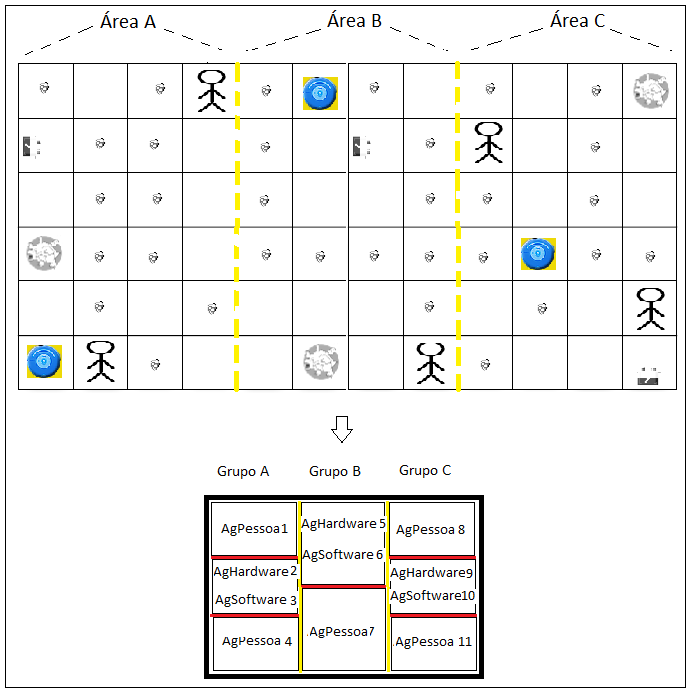
\includegraphics[width=8cm]{figuras/asp-estrutura.png}
        }{
            \Fonte{Elaborado pelo autor.}
        }   
    \end{figure}
    \clearpage
    A Tabela \ref{tab:org-estrutura} apresenta o modelo $E$ para a organização esboçada na Figura \ref{fig:asp-estrutura}. Ela mostra um conjunto de onze programas de agentes, divididos em três grupos, cada grupo responsável por uma área do ambiente. A tabela apresenta apenas algumas relações do tipo Conhecimento, omitindo-se as relações de Controle, Coordenação e Autoridade existentes entre os papéis que podem ser exercidos pelos programas.
    
    \begin{table}[h!]   
        \centering
        \Caption{\label{tab:org-estrutura} Organização dos agentes de acordo com o modelo de estrutura.}
        \UECEtab{}{
            \begin{tabular}{| p{5cm} | p{10cm}|}
            \hline
            \textbf{Agent} & \{$AgPessoa_1$, $AgHardware_2$, $AgSoftware_3$, $AgPessoa_4$, $AgHardware_5$, $AgSoftware_6$, $AgPessoa_7$, $AgPessoa_8$, $AgHardware_9$, $AgSoftware_{10}$, $AgPessoa_{11}$\} \\ \hline
            
            \textbf{Roles} & \{User, Device, Controller\}                                       \\ \hline
            
            \textbf{AgentRoles} & \{AgentAmIUser, AgentAmIDevice, AgentAmIController\}   \\ \hline
            
            AgentAmIUser & \{$AgPessoa_1$, $AgPessoa_4$, $AgPessoa_7$, $AgPessoa_8$\}   \\ \hline
            
            AgentAmIDevice & \{$AgHardware_2$, $AgHardware_5$, $AgHardware_9$\}         \\ \hline
            
            AgentAmIController & \{$AgSoftware_3$, $AgSoftware_6$, $AgSoftware_{10}$\}  \\ \hline
             
              
            \textbf{Groups} & \{\{$AgPessoa_1$, $AgHardware_2$, $AgSoftware_3$, $AgPessoa_4$\}, \{$AgHardware_5$, $AgSoftware_6$, $AgPessoa_7$\}, \{$AgPessoa_8$, $AgHardware_9$, $AgSoftware_{10}$, $AgPessoa_{11}$\}\} \\ \hline 
            
            \textbf{Bond} & \{$Bond_{knowledge}$(AgentAmIUser, AgentAmIDevice), \newline $Bond_{knowledge}$(AgentAmIDevice, AgentAmIController)\}    \\ \hline
            
             $Bond_{knowledge}$(AgentAmIUser, AgentAmIDevice) & \{($AgPessoa_1$, $AgHardware_2$), ($AgPessoa_4$, $AgHardware_2$), ($AgPessoa_7$, $AgHardware_5$), ($AgPessoa_8$, $AgHardware_9$), ($Agpessoa_{11}$, $AgHardware_9$), \dots \};  \\ \hline
        
             $Bond_{knowledge}$(AgentAmIDevice, AgentAmIController) & \{($AgHardware_2$, $AgSoftware_3$), ($AgHardware_5$, $AgSoftware_6$), ($AgHardware_9$, $AgSoftware_{10}$)\}  \\ \hline
             
             \vdots & \vdots \\ \hline

            \textbf{Communication} & \{($AgPessoa_1$, $AgHardware_2$), ($AgPessoa_1$, $AgHardware_5$), ($AgHardware_2$, $AgSoftware_3$), ($AgHardware_2$, $AgPessoa_4$), ($AgHardware_2$, $AgHardware_5$), ($AgHardware_2$, $AgPessoa_7$), \ldots \} \\ \hline
            
            \textbf{Frequency} & Ilustrado na Figura \ref{fig:matriz-decomponivel} \newline \\

            \hline
            \end{tabular}
        }{
        \Fonte{Elaborado pelo autor}
    }
    \end{table}
    
    
    Os programas de agentes $AgPessoa_1$, $AgPessoa_4$, $AgPessoa_7$, $AgPessoa_8$ e $AgPessoa_{11}$ são programas empregados para representar pessoas. Esses agentes exercem o papel de usuários do prédio (\textit{User}), que são capazes de caminhar em direção a qualquer local desejado. 
    
    Os programas de agentes $AgHardware_2$, $AgHardware_5$ e $AgHardware_9$, são programas empregados para representar o \textit{hardware} dos sistemas técnicos no sistema \acrshort{ami}. Estes programas exercem o papel de sensores e/ou de atuadores (\textit{Devices}), capazes de perceber o ambiente, movimentar um aspirador e aspirar sujeira, além de interagir com os programas do tipo $AgPessoas$.
    
    Os programas de agentes $AgSoftware_3$, $AgSoftware_6$ e $AgSoftware_{10}$ são programas que implementam os componentes do \textit{software} no sistema técnico do sistema \acrshort{ami}. Esses programas exercem o papel de controladores (\textit{Controller}) capazes de interagir com os agentes $AgHardware$, requisitando informações dos sensores e indicando ações adequadas para serem executadas pelos atuadores no ambiente.
    
    A segunda parte do modelo $E$ foca no componente da estrutura organizacional que descreve formalmente o mapa das interações entre os agentes na organização. Este mapa contém dois tipos de informações: (1) a relação $Communication$ na Tabela \ref{tab:org-estrutura} informa quem pode enviar mensagem para quem, dentro de um mesmo grupo e entre grupos diferentes de programas de agentes na organização; (2) a matriz sociométrica $Frequency$, ilustrada na Figura \ref{fig:matriz-decomponivel}, informa a frequência com que os programas de agentes trocam mensagens entre si, isto é, a frequência que, em geral, é necessária para dar suporte às relações binárias existentes entre os programas (Conhecimento, Controle, Coordenação e Autoridade) em diferentes papéis na organização. 
        
    \begin{figure}[h!]
        \centering
        \Caption{\label{fig:matriz-decomponivel} Mapa das interações entre os programas de agentes de diversos grupos.} 
        \UECEfig{}{
            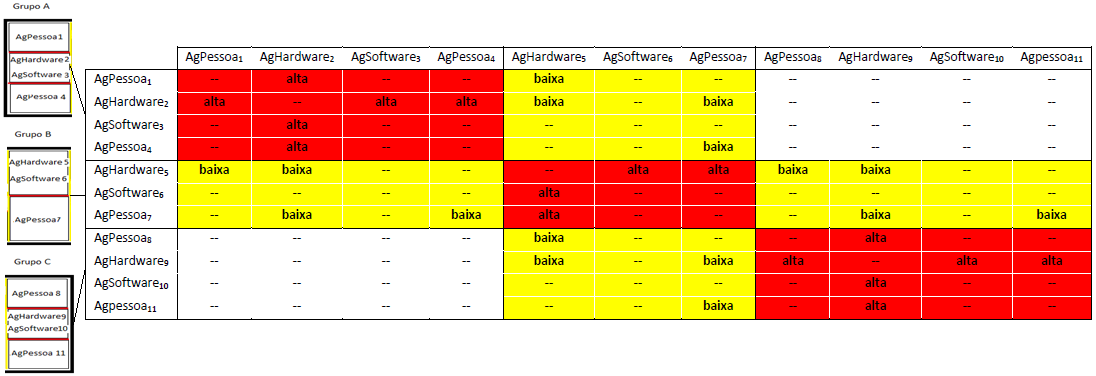
\includegraphics[width=12cm]{figuras/matriz-decomponivel.png}
        }{
            \Fonte{Elaborado pelo autor.}
        }   
    \end{figure}
    
    A matriz sociométrica acima informa a frequência $f_{xy}$ com que cada par de programas de agentes $(AgentAmI_x, AgentAmI_y) \in Communication$ trocam mensagens entre si. A matriz permite informar também as concentrações de interações densas, ou seja, programas de agentes em um mesmo grupo estão agrupados na matriz, de forma que as células que possuem os maiores valores de frequência ficaram numa linha de submatrizes quadradas ao longo da diagonal principal e todos as células fora destes quadrados da diagonal têm valores de frequência zero ou muito pequeno.    
    
    Nesse tipo de estrutura organizacional quase decomponível é possível distinguir as trocas de mensagens entre grupos de agentes (amarelo) e as trocas dentro dos grupos (vermelho). Nessas organizações, as trocas de mensagens entre grupos são menos frequentes, mas não são desprezíveis. Assim, se dois agentes -- $AgentAmI_x$ e $AgentAmI_y$ -- estiverem em um mesmo grupo e existir uma “parede” comum entre eles, então, a frequência da troca de informações entre eles será: $f_{xy} = alta$. E se os agentes estiverem em grupos diferentes e existir uma parede separando-os, então, a frequência será: $f_{xy} = baixa$ (ou, dependendo do caso, $f_{xy} = media$).
    
    Assim, considerando que a maioria dos sistemas \acrshort{ami} pode ser descrita por organizações de programas de agentes em uma estrutura quase decomponível, o projetista pode agir de duas maneiras diferentes, considerando as ideias implícitas no modelo E. Ele pode empregar a primeira parte do modelo para formalizar previamente os grupos de agentes na organização e, em seguida, empregar a segunda parte do modelo para formalizar o mapa de interações sociais em função dos grupos formalizados. Mas ele pode também formalizar previamente o mapa de interações entre os agentes e, em seguida, formalizar os grupos operacionalmente considerando uma medida de frequência de interação no mapa. 
    
    
    \subsection{Modelo de Comportamento (C)}
    
        Depois de se concentrar na descrição estrutural, empregando o modelo $E$ da organização de programas de agentes representando o sistema \acrshort{ami}, o projetista deve ser capaz de descrever como a estrutura projetada deve funcionar (comportamento) para realizar o objetivo original do sistema, sua função descrita no modelo $F$, no ambiente de tarefas. O modelo de comportamento (modelo $C$) permitirá a descrição formal de procedimentos de tomada de decisão nos programas de agentes, em seus papéis na organização e nos processos que ocorrem dentro da organização, definindo como os programas de agentes, integrados na estrutura organizacional, devem agir de maneira a alcançar os resultados desejados.
        
        O quadro formal que define o modelo $C$ pode ser dividido em duas partes. A primeira parte permitirá ao projetista determinar os “esqueletos” dos programas de agentes, definidos no conjunto $Agents$ do modelo $E$. Estes "esqueletos" de programa deverão ser customizados de acordo com os papéis que assumirão em um domínio específico de aplicação. Essa customização implica na definição do conjunto de comportamentos que cada programa deve ser capaz de executar quando adotar algum papel na organização -- no modelo $E$, aqueles papéis definidos no conjunto $Roles$. A segunda parte do quadro permitirá ao projetista definir o protocolo de interação descrevendo as trocas de mensagens possíveis -- no modelo $E$, descritas na relação $Communication$ --, visando coordenar as ações dos programas em seus papéis na organização.
        
        \subsubsection{Descrição Formal dos “Esqueletos” de Programas de Agentes}
        
            No nível individual, o modelo $C$ permitirá ao projetista descrever formalmente os esqueletos dos programas de agentes na organização. Cabe ao projetista definir a especificação do conjunto de comportamentos a serem incorporados nesses esqueletos, que devem ser adequados aos papéis $R_j \in Roles$ que os programas nos conjuntos $AgentAmIRj \in AgentRoles$, descritos no modelo $E$, devem assumir no domínio de aplicação de interesse do projetista. O formalismo para descrição desses esqueletos foi sintetizado a partir dos trabalhos de \citeonline{norvig2004inteligencia}, sobre estruturas de programas de agentes, e de \citeonline{wooldridge2009introduction}, sobre arquiteturas abstratas de agentes. A Figura \ref{fig:estrutura-agente} ilustra graficamente a estrutura e os esqueletos de pelo menos quatro tipos diferentes de programas de agentes resultantes dessa síntese.
            
            Mais especificamente, a figura ilustra um refinamento em duas etapas do subsistema de tomada de decisão, $ação: S^*  \rightarrow A$ (função que mapeia sequências de estados do ambiente $s \in S^*$ em ações $a \in A$), apresentada na seção que descreve o quadro formal associado ao modelo $F$ da organização. À esquerda, o primeiro refinamento dando origem ao subsistema de percepção do agente. À direita, o segundo refinamento dando origem ao subsistema de estado interno do agente. O primeiro refinamento apresenta a arquitetura e o esqueleto de programas de agentes reativos simples baseados em regras condição-ação. O segundo refinamento apresenta a arquitetura e o esqueleto de programas de agentes reativos baseados em modelos, orientados por objetivos e por metas, dependendo do tipo de informação ($InfoDecisão$) que o projetista desejar incorporar ao processo de tomada de decisão (regras, objetivos, utilidades).
            
            \begin{figure}[h!]
                \centering
                \Caption{\label{fig:estrutura-agente} Estrutura dos programas de agente.} 
                \UECEfig{}{
                    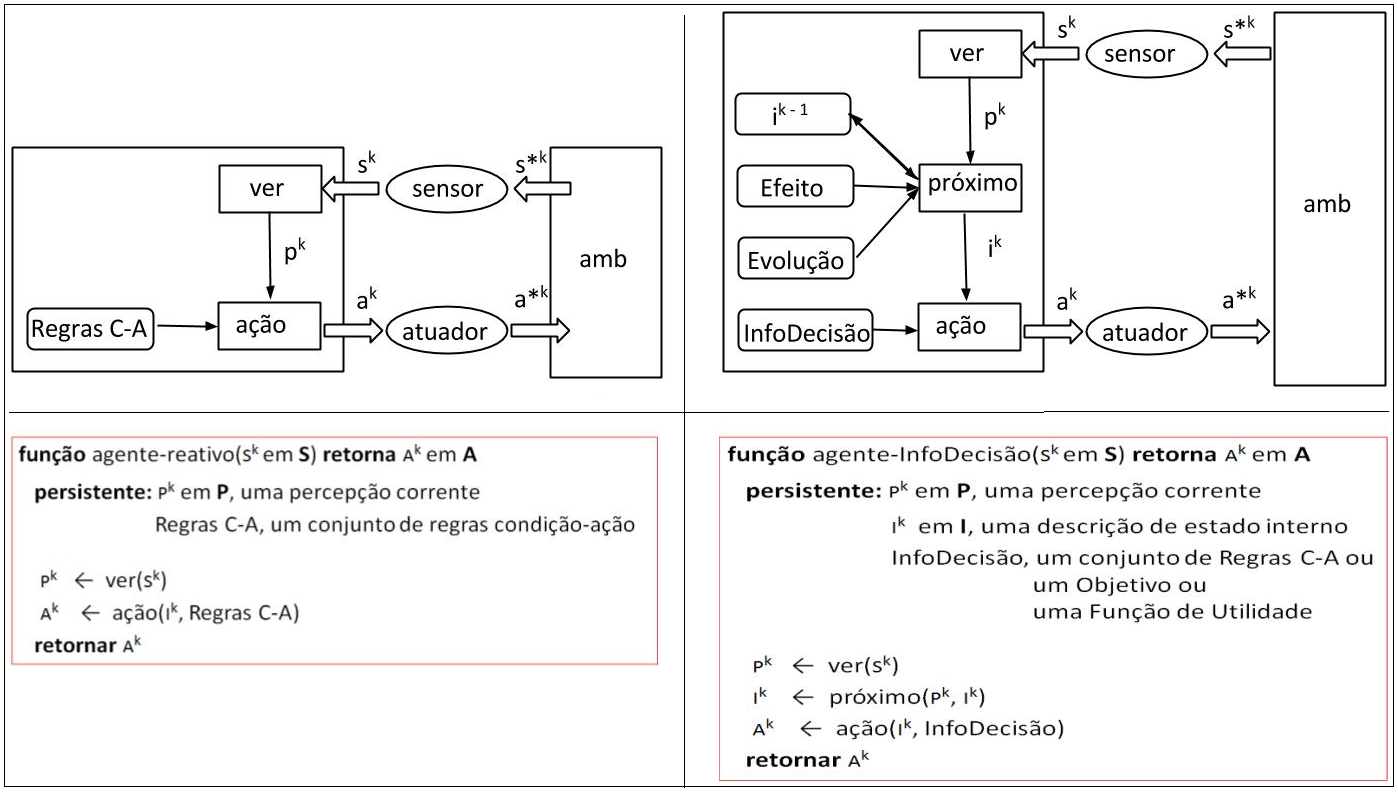
\includegraphics[width=12cm]{figuras/estrutura-agente}
                }{
                    \Fonte{Elaborado pelo autor.}
                }   
            \end{figure}
            
            Além de serem empregados na concepção de programas de agentes para representar pessoas e o \textit{software} do sistema, esses esqueletos devem ser utilizados também na concepção de programas de agentes, para representar o \textit{hardware} do sistema. Esses agentes são ilustrados na Figura \ref{fig:estrutura-agente} como elipses, com os nomes sensor e atuador, conforme ilustram os esqueletos de agentes reativos simples empregados para representar estes componentes do \textit{hardware} nos sistemas técnicos ilustrados na Figura \ref{fig:org-level-p4}. O quadro apresentado na Tabela \ref{tab:def-prog-agent} consiste em uma extensão do quadro inicialmente desenvolvido no modelo $F$, o qual apresenta o esquema de representação e a definição correspondente dos principais termos envolvidos na definição dos esqueletos de programas de agentes ilustrados na Figura \ref{fig:estrutura-agente}.
            
            \begin{table}[h!]   
            \centering
            \Caption{\label{tab:def-prog-agent} Definição dos termos envolvidos no esqueleto do programa de agente.}
            \UECEtab{}{
                \begin{tabular}{| p{4cm} | p{10cm}|}
                \hline
                $P = \{P_1, P_2, \ldots \}$ & Percepção do ambiente do agente - em qualquer instante o agente recebe por meio de sensores entradas perceptivas em um conjunto de percepções do ambiente;\\ \hline
                
                $ver: S  \rightarrow P$ & Subsistema de percepção do programa - captura a habilidade do agente observar seu ambiente, uma função que mapeia estados do ambiente para percepções;      \\ \hline
                
                $I = \{I_1, I_2, \ldots \}$ & Estados internos do ambiente - em qualquer instante o agente mantém em memória uma descrição de estado em um conjunto de estados interno do ambiente;   \\ \hline
                
                próximo: $I\times P \rightarrow I$ & Subsistema de atualização de estado interno do programa – função que mapeia um estado interno e a percepção atual, que chega da função ver, em um estado interno;   \\ \hline
                
                ação: $I \rightarrow A$ & Subsistema de tomada de decisão do programa – função que mapeia estados internos em ações.         \\ \hline
                
                $Sucessor: I \rightarrow P(I \times A)$ & Efeito das ações do agente no ambiente – função que mapeia um estado interno em um conjunto de pares estado interno e ação;   \\ \hline
                 
                Ações: $I \rightarrow 2^A$ & Conjunto de ações possíveis para o agente em um estado – mapeia um estado interno em um conjunto de ações possíveis de serem executadas no estado;  \\ \hline
                
                $RESULTADO: I \times A \rightarrow I$ & Modelo de transição – descrição formal do que cada ação faz, uma função que mapeia um estado interno e uma ação em um novo estado interno; \\ \hline
            
                Meta:$I \rightarrow \{V,F\}$ & Função que mapeia uma descrição de estado interno em um valor verdade;  \\ \hline
                 
                $Utilidade: I \rightarrow \mathbb{R}$ & Função que mapeia uma descrição de estado interno em um valor real. \\ 
                \hline
                \end{tabular}
            }{
            \Fonte{Elaborado pelo autor}
        }
        \end{table}
        
        Em resumo, à esquerda na Figura \ref{fig:estrutura-agente}, um programa agente reativo simples seleciona suas ações baseando-se apenas em sua percepção atual e em um conjunto de regras no formato condição-ação. À direita na Figura \ref{fig:estrutura-agente}, um programa agente reativo baseado em modelos mantém internamente em memória uma descrição de estado de seu ambiente, o qual depende do histórico de suas percepções. Essa mesma figura pode representar um programa agente orientado por objetivos, que, além das informações em memória, considera a informação sobre os objetivos que descrevem situações desejadas no ambiente. O programa do agente orientado por utilidade possui uma função utilidade que mapeia uma descrição de estado do ambiente em um grau de felicidade associado. 
    
        O subsistema de atualização de estado interno (próximo) dos agentes reativos baseados em modelos, orientados por objetivos e por utilidade, e o subsistema de tomada de decisão (ação) dos dois últimos, em comum, processam informações de dois tipos, ou seja: sobre como o ambiente evolui independentemente das ações do agente (Evolução) e sobre o efeito das ações do agente no ambiente (Efeito). A utilização dessas informações nos dois subsistemas pode ser representada por meio de uma função Sucessor de estado, e/ou por meio das funções \emph{Ações} e \emph{RESULTADO} no quadro.
        
        As informações sobre o objetivo, processadas pelo subsistema de tomada de decisão do agente orientado por objetivo, é representada por um teste Meta. Quando verdadeiro, esse teste diz ao agente que ele pode parar o seu processo de deliberação. De forma semelhante, o agente orientado por utilidade deve empregar uma função utilidade, do tipo especificado no modelo $F$, para medir a qualidade dos estados realizados por ações que ele tenha como alternativas.
        
        O algoritmo \ref{alg:decision-function} descreve uma função tomada de decisão de um programa de agente aspirador de pó, do tipo $AgSoftware$, no papel Controlador. O programa deve ser capaz de controlar o aspirador visando varrer uma área e aspirar aqueles locais que contém sujeira. O aspirador deve realizar um movimento horizontal (direita ou esquerda) na área enquanto não perceber sujeira e obstáculos. Quando perceber que existe um obstáculo (parede ou pessoa), impossibilitando-o de realizar um movimento, o aspirador deve realizar um movimento vertical para cima/baixo (girar $90^\circ$ no sentido anti-horário e seguir em frente). Em seguida, modificar a direção horizontal (esquerda/direita e vice-versa) e seguir em frente em busca de novos locais contendo sujeira.
        
        \begin{algorithm}[h!]
            %\SetSpacedAlgorithm
            \caption{\label{alg:decision-function} Descrição parcial da função tomada de decisão de um agente reativo.}
            %\Entrada{$p^k$ em S}
            %\Saida{$a^k$ em A}
            função ação ($p^k$ em S) retorna $a^k$ em A\\
            \Inicio{
                \ldots\\
                \textbf{se} $p^k$ = obstáculo \textbf{então} \textbf{retornar} $a^k$ = aspirar\;
                \textbf{senão se} $p^k$ = obstáculo \textbf{então} \textbf{retornar} $a^k$ = rotacionar $90^\circ$ esquerda\;
                \textbf{senão se} $p^k$ = limpo \textbf{então} \textbf{retornar} $a^k$ = frente\;
                \ldots\\
            }
        \end{algorithm}
        
        A função tomada de decisão diz respeito a um programa de um agente do tipo reativo simples baseado em regras de condição-ação. As expressões que definem as condições nas regras são estabelecidas levando-se em consideração as informações no conjunto de percepções do ambiente que são possíveis para o agente $P = \{P_1, P_2, \ldots \}$. Os programas de agentes baseados em modelos são mais adequados para ambientes parcialmente observáveis. Eles podem empregar as informações que descrevem o estado interno, $I = \{I_1, I_2, \ldots \}$, para evitar retornar em locais por onde já passaram. E, ainda, evitar passar em locais que foram visitados recentemente por outros agentes, através de um processo cooperativo de troca de mensagens em um sistema composto por mais de um aspirador.
    
    \subsubsection{Descrição Formal do Protocolo de Interação Global Entre os Agentes}
    
        Na subseção anterior, descrevemos a parte do modelo $C$ que representa o comportamento interno de um agente. Mas essa parte do modelo só é capaz de descrever sistemas que contenham agentes únicos. Em vez de um sistema \acrshort{ami} formado por um único aspirador, vale considerar a situação em que um grupo de aspiradores são capazes de cooperar uns com os outros. Os agentes podem trocar mensagens contendo informações úteis sobre o ambiente de tarefas, visando alcançar da melhor maneira o objetivo original do sistema. 
        
        O processo de comunicação e intercâmbio de conhecimento é conhecido como cooperação. Dependendo do ambiente de tarefas, a cooperação pode ser um requisito crucial. Por exemplo, cada agente pode cooperar utilizando a operação coletiva \textit{broadcast}, ou seja, operação de transmissão de uma mesma mensagem para todos os outros agentes no grupo. 
    
        A ideia é que, para alcançar seus objetivos e o objetivo original do sistema, os agentes componentes possam se comunicar através de uma linguagem de comunicação em que os atos de fala são visualizados como ações (da mesma forma que as ações executadas pelos atuadores do agente), cujos efeitos ocorrem principalmente nos modelos que os falantes e os ouvintes mantêm uns dos outros. Neste contexto, os atos de fala dos agentes podem ser integrados nos processos de atualização de estado interno (informação sobre efeito de um ato) e de tomada de decisão dos programas de agentes (por exemplo, como consequentes em regras condição-ação). 
        
        A segunda parte do modelo $C$ foca na descrição do quadro formal, que pode ser adaptado para definir o protocolo de comunicação entre os agentes em um mesmo grupo e entre os agentes em grupos diferentes na organização. A abordagem considera que os agentes são capazes de trocar mensagens por meio de canais de comunicação. Cada agente atua assincronamente monitorando uma fila de mensagens de entrada, que chegam pelo canal, e enviando mensagens para uma fila de saída, que serão transmitidas pelo canal para um ou mais agentes.
        
        A principal parte do quadro proposto para a segunda parte do modelo $C$ consiste em uma variação do quadro empregado para a definição formal da noção de autômatos de estados finitos (\acrshort{afd}). O quadro resultante empresta algumas ideias implementadas no formalismo para a especificação de cenas em instituições eletrônicas \cite{vasconcelos2002approach}, baseado na noção de autômatos finitos não determinísticos. No modelo $C$, um protocolo de interação entre agentes é descrito como um \acrshort{afd}, onde os estados representam diferentes estágios de conversação e os arcos direcionados, conectando os estados, são rotulados com mensagens escritas em uma linguagem de comunicação, ou com alguma condição descrita em termos de um período de tempo entre dois instantes consecutivos de transmissão de mensagens no processo de conversação. Ou seja:
        
        \newtheorem{theorem}{Definição}

        
        \begin{theorem}
            Protocolo = $(T, LC, Q, q_0, \delta, G)$, tal que:
            \begin{itemize}
                \item T = \{$t_1$, \ldots, $t_m$\} - um conjunto discreto e parcialmente ordenado de instantes, para marcar a transmissão de mensagens em um processo de conversação;
                \item LC – linguagem empregada para a comunicação entre os agentes;
                \item Q – conjunto de estados possíveis do protocolo (é finito);
                \item $q_0 \in Q$ – estado inicial do protocolo;
                %\item $F \subset Q$ - conjunto de estados finais do protocolo; % NAO EXISTE MAIS
                \item $\delta$ – função programa ou função transição (função parcial) – associa estados em $Q$ e mensagens em $LC$, ou uma condição descrita em termos de T, a estados em $Q$, ou seja, $\delta$: $Q$ $\times$ ($LC$ $\cup$ condição(T)) $\to$ $Q$;
                \item $G \subset P(Agentes)$ – família de conjuntos de agentes que podem participar do processo de conversação especificado no protocolo.
            \end{itemize}
        \end{theorem}
        
        A especificação de um protocolo de comunicação entre um grupo de agentes $G$ considera um único estado inicial $q_0$. Apesar de não existirem estados finais, o estado inicial também representa as diferentes possibilidades de um agente finalizar uma conversação. Com relação à linguagem para comunicação ($CL$), o modelo $C$ considera uma linguagem de atos de fala que podem ser gerados a partir de dois atos de fala considerados como mensagens fundamentais: $request$ e $inform$. A Figura \ref{fig:inform-request} ilustra o formato proposto para estas mensagens e dois exemplos de composições destas mensagens visando gerar atos de fala de perguntas (\textit{requests to inform}) e solicitações envolvendo pelo menos três agentes (\textit{requests to request}). 
    
        \begin{figure}[h!]
            \centering
            \Caption{\label{fig:inform-request} Troca de mensagens entre os agentes da organização.} 
            \UECEfig{}{
                \includegraphics[width=8cm]{figuras/inform-request}
            }{
                \Fonte{Elaborada pelo autor.}
            }   
        \end{figure}
            
        Cada mensagem transmitida deve conter representações de informações sobre a intenção da mensagem dos agentes falantes ($S$) e os ouvintes ($H$), assim como sobre o conteúdo da mensagem a ser trocada entre os agentes ($Action$ ou $Statement$) e o instante ($t$) da conversação. Qualquer agente falante $S$ que envia uma mensagem do tipo $request$ objetiva fazer com que algum agente ouvinte $H$ execute uma ação $Action$. Qualquer agente falante $S$ que envia uma mensagem do tipo $inform$ objetiva fazer com que o agente ouvinte $H$ acredite em alguma afirmação ($Statement$). Assim como no caso da formulação de mensagens envolvendo questões, toda a semântica dos atos de fala que compõem a linguagem de comunicação \acrshort{fipaacl} (\acrlong{fipaacl}) pode ser definida em termos de $inform$ e $request$.
        
        Para ilustrar a formalização da noção de protocolos, vale considerar o exemplo do grupo de aspiradores capazes de cooperar uns com os outros, visando limpar o ambiente no menor tempo possível. Por exemplo, cada agente pode cooperar utilizando a operação coletiva \textit{broadcast}, transmitindo uma mesma mensagem para todos os outros agentes no grupo. Assim, quando perceber um local (célula) contendo sujeira, o agente pode transmitir a posição da célula e a quantidade de sujeira aos outros. Quando a mensagem for recebida, cada agente pode armazenar as informações no estado interno e, em seguida, decidir se vai em direção ao local, avisando ou não ao agente que enviou a mensagem. Quando limpar uma célula, o agente pode transmitir esta informação novamente para os outros agentes no grupo. Quando a mensagem for recebida, o agente pode remover do estado interno a informação sobre sujeira na célula que foi limpa.
        
        \clearpage
        A Figura \ref{fig:protocolo-transicao} descreve graficamente uma parte da função transição ($\delta$) componente do protocolo de comunicação entre os agentes. O protocolo considera um conjunto de dois estados possíveis, $Q$ = \{$q_0$, $q_1$\}, com o estado inicial representado por $q_0$. A figura supõe que o processo de conversação envolve uma família formada por um conjunto contendo os programas no papel Controller, isto é, G = {AgentAmIController} (como G é unitário, em vez de fazer referência ao conjunto AgentAmIController, a figura faz referência à própria família G).
            
        \begin{figure}[h!]
            \centering
            \Caption{\label{fig:protocolo-transicao} Protocolo de transição.} 
            \UECEfig{}{
                \includegraphics[width=8cm]{figuras/protocolo-transicao}
            }{
                \Fonte{Elaborada pelo autor.}
            }   
        \end{figure}
       
        Na primeira etapa do processo de conversação, no instante $t_1$, representada pelo componente da função transição $\delta$($q_0$, $inform(\ldots, t_1)) = q_1$, um agente falante s $\in$ G pode enviar sua posição ($x_1$, $y_1$) e a quantidade de sujeira z na posição para todos os outros agentes ouvintes h $\in$ G. Na segunda etapa, no instante $t_2$, alguns dos agentes ouvintes podem responder a mensagem dizendo se definiram, ou não, a posição ($x_1,y_1$) como meta, $\delta$($q_1$, $inform(\ldots, t_2) = q_0$. Entretanto, os agentes podem não enviar mensagem de retorno. Neste caso, depois de $\epsilon$ unidades de tempo, contadas a partir do horário de início da conversação no instante $t_1$ (tempo($t_1$)) até um tempo limite em que uma mensagem de retorno deve ser enviada no instante $t_2$ (tempo($t_2$)), o protocolo transita para o estado inicial, $\delta$($q_1$, tempo($t_2$) – tempo($t_1$) > $\epsilon$, $t_2$) = $q_0$, em que os agentes poderão iniciar novo processo de conversação.
        
        Conforme ilustra o mapa das iterações sociais na Figura \ref{fig:matriz-decomponivel}, a descrição parcial da função transição omitiu as trocas de mensagens que existem entre os agentes no papel $AgentAmIDevice$ e os agentes no papel $controller$. Estas trocas ocorrem com muita frequência e, assim como possíveis trocas entre os agentes no papel $AgentAmIDevice$ com os agentes no papel $AgentAmIUser$, devem ser especificadas de maneira a completar a definição do protocolo de interação global entre todos os agentes no grupo exemplificado.
        
\end{section}

\section{Considerações Finais}

    A proposta \textbf{P6}, escrita na introdução deste capítulo, consiste na utilização de simulação computacional baseada em agentes (\acrshort{ads}) como um meio para examinar a dinâmica de um sistema \acrshort{ami}. A \acrshort{ads} permitirá ao projetista experimentar diversos contextos operacionais do sistema \acrshort{ami}, possibilitando a aquisição de novos conhecimentos sobre o funcionamento do sistema em seu ambiente, e outras formas de adaptar o seu modelo estrutural ($E$) e o comportamental ($C$),  visando melhorar o desempenho do sistema quando for necessário, de acordo com o que for especificado no modelo $F$.
    
    Conforme a Figura \ref{fig:sim-emergente-p6} (na seção de introdução deste capítulo) indica, a execução de uma simulação considera como informações de entrada, o modelo \acrshort{fec} do sistema \acrshort{ami}, o modelo do ambiente de tarefas e os valores dos parâmetros de entrada. Descrevendo um contexto operacional de funcionamento do sistema no ambiente, a execução de uma \acrshort{ads} deve gerar como saída as informações sobre o desempenho do sistema conforme descrito no modelo $F$. Essas informações de desempenho, ou objetos emergentes, são resultado das interações descritas no modelo $C$, executadas por programas de agentes na organização estruturada no modelo $E$. 
    
    Uma execução pode ser vista como uma dedução de alguma informação sobre o sistema \acrshort{ami} sendo projetado. Uma coleção destas deduções, obtidas metodicamente pela execução de várias \acrshort{ads}, pode ser vista como a informação necessária para o projetista realizar inferências (indutivas) sobre o comportamento do sistema, permitindo a ele deduzir se o sistema será capaz de realizar o objetivo original em seu ambiente de tarefas.
    